\documentclass[../sparc.tex]{subfiles}
\graphicspath{{\subfix{../images/}}}
\begin{document}

%%%%%%%%%%%%%%%%%%%%%%%%%%%%%%%%%%%%%%%%%%%%%%%%%%%%%%%%%%%%%%%%%%%%%%%%%%%%%%%%
\section{Аналогово-цифровое преобразование}
\newglossaryentry{АЦП}{name=АЦП, description={Аналогово-Цифровой Преобразователь}}
\newglossaryentry{ЦАП}{name=ЦАП, description={Цифро-Аналоговый Преобразователь}}
\newglossaryentry{ADC}{
  name=ADC,
  description={Analog-to-Digital Converter (см. \gls{АЦП})}}
\newglossaryentry{DAC}{
  name=DAC,
  description={Digital-to-Analog Converter (см. \gls{ЦАП})}}


Мы могли заметить в главе \ref{section:analog-ports}, что при считывании с
аналогово порта получается значения в диапазоне от 0 до 1023.  Число 1023
подозрительно похоже на число 1024, которое в программировании встречается
достаточно часто -- не удивительно, ведь 1024 это степень двойки ($2^{10}$).

Давайте разберёмся, почему же значения с аналогового порта в Arduino находятся
именно в таком диапазоне.  Начнём с того, что аналоговый порт каким-то образом
преобразует входящий аналоговый сигнал в цифровое (двоичное) представление,
которое мы и видим в программе.

Операцию преобразования аналогового сигнала в цифровой выполняет компонент,
называемый \emph{Аналого-Цифровой Преобразователь} (сокращённо \gls{АЦП}.)  В
роли АЦП может выступать как отдельная микросхема, так и сам микроконтроллер.
Схематически аналогово-цифровой преобразователь можно изобразить, как показано
на рис. \ref{fig:adc-schematics}.

По-английски ``АЦП'' -- ``Analog-to-Digital Converter'' (сокращённо \gls{ADC}.)

\begin{figure}[ht]
  \centering
  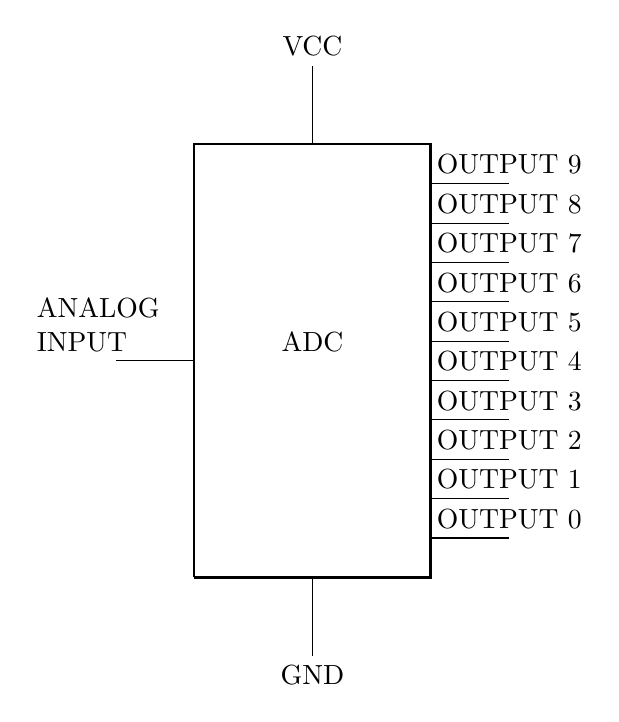
\begin{tikzpicture}
    \draw[thick] (0, 0) -- (0, 5.5) -- (3, 5.5) -- (3, 0) -- (0, 0);
    \draw (1.5, 2.75) node[right, above] {ADC};
    \foreach \n/\y in {0/0.5, 1/1, 2/1.5, 3/2, 4/2.5, 5/3, 6/3.5, 7/4, 8/4.5, 9/5} {
      \draw (3, \y) -- (4, \y) node[right, above] {OUTPUT \n};
    };
    \draw (0, 2.75) -- (-1, 2.75) node[left, above, text width=2cm] {ANALOG INPUT};
    \draw (1.5, 5.5) -- (1.5, 6.5) node[right, above] {VCC};
    \draw (1.5, 0) -- (1.5, -1) node[right, below] {GND};
  \end{tikzpicture}
  \caption{Схематическое изображение аналогово-цифрового преобразователя.}
  \label{fig:adc-schematics}
\end{figure}

На вход АЦП (``ANALOG INPUT'') подаётся аналоговый сигнал, а на выходах
(``OUTPUT 0'' .. ``OUTPUT 9'') кодируется значение входного сигнала в каждый
момент времени в виде набора логических уровней ``HIGH'' (``1'') / ``LOW''
(``0''.)  Самому АЦП требуется также питание -- для этого как раз предназначены
выводы ``VCC'' и ``GND''.

\example { На вход АЦП подаётся 2.5В.  На выходах формируется двоичное значение
  ``1000000000'', что соответствует числу $2^9 = 512$, которое может быть
  получено в программе микроконтроллера. }

Преобразование аналогового сигнала в цифровой внутри АЦП проходит в три этапа:
\begin{enumerate}

\item \textbf{Дискретизация.} Выбираются значения из исходного аналогового сигнала через
  равные временные промежутки (\ref{fig:discretization}.)

  \begin{figure}[h]
    \centering
    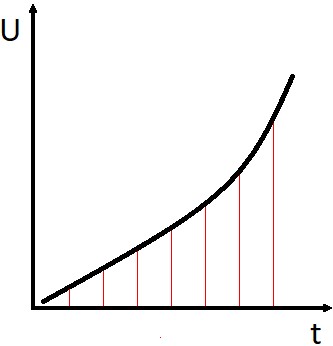
\includegraphics[width=8cm]{discretization}
    \caption{Дискретизация.}
    \label{fig:discretization}
  \end{figure}

  Характеристика, отражающая эти временные промежутки, называется \emph{частотой
  дискретизации}.

\item \textbf{Квантование.} Полученные значения заменяются ближайшим значением из
  набора фиксированных величин -- \emph{уровней квантования}
  (\ref{fig:quantization}.)

  \begin{figure}[h]
    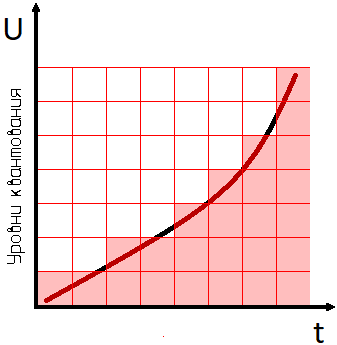
\includegraphics[width=8cm]{quantization}
    \caption{Квантование.}
    \label{fig:quantization}
    \centering
  \end{figure}

\item \textbf{Кодирование.} Квантованным значениям присваивается цифровой код
  (\ref{fig:coding}.)

  \begin{figure}[h]
    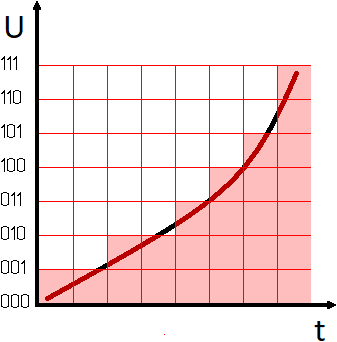
\includegraphics[width=8cm]{coding}
    \caption{Кодирование.}
    \label{fig:coding}
    \centering
  \end{figure}

  Чем выше частота дискретизации и чем больше уровней квантования, тем точнее
  преобразование.

\end{enumerate}

Одной из характеристик АЦП является \emph{разрядность}.  Она определяет диапазон
значений, которое может выдать АЦП.

Компьютеры оперируют двоичной системой исчисления -- то есть, минимальная единица
хранения информации, называемая \emph{бит}, может хранить только одно из двух
значений: один или ноль.

В двух подобных ячейках (битах) мы можем хранить уже 4 комбинации нулей и
единиц: 00, 01, 10, 11.  Если мы возьмём 3 бита, то это даст нам уже 8
комбинаций.  Несложно проследить зависимость: добавление каждого дополнительного
бита увеличивает количество комбинаций в два раза.

Это можно посчитать даже проще: нам не нужно вручную вписывать единицы и нули в
условные ``клетки'' и считать их.  Вместо этого мы можем использовать следующую
формулу:

\begin{equation}
  \mbox{количество комбинаций} = 2^{\mbox{n}}
\end{equation}

Где \texttt{n} -- это количество бит, доступных для хранения значения.

Для примера, если мы возьмём 8 бит для хранения информации, то это даст нам $2^8
= 256$ комбинаций нулей и единиц.

Посмотрим на график (\ref{fig:coding}): для кодирования значений используется
три бита -- значит АЦП, описываемый таким графиком, имеет разрядность 3 бита.  То
есть, количество уровней квантования будет $2^3 = 8$.

Однако нам надо не забывать, что отсчёт в компьютерном мире обычно ведётся с
нуля, и ситуация, когда все биты выставлены в ноль, тоже является одним из
доступных значений диапазона.  Предположим, что нам доступно 8 бит и мы их все
задали, равными единице, то есть $11111111_2$.  Если мы переведём это число в
десятичную форму, то получим:

\begin{equation}
  11111111_2 = (2^7 * 1) + \mbox{...} + (2^2 * 1) + (2^1 * 1) + (2^0 * 1) = 255_{10}
\end{equation}

Таким образом мы видимо, что максимальное положительное значение для 8 бит равно
числу 255.

Из этого оследует, что максимальное значение для \texttt{n} бит можно посчитать
по следующей формуле:

\begin{equation}
  \mbox{максимальное значение} = 2^{\mbox{n}} - 1
\end{equation}

Из этого следует, что если мы возьмём 10 бит для хранения информации, то в них
мы можем закодировать 1024 комбинаций из нулей и единиц, так как $2^{10} =
1024$.  Но максимальное положительное значение будет равно 1023.  Следовательно
в Arduino АЦП имеет разрядность 10 бит.

Также ещё есть такое устройство как \emph{Цифро-Аналоговый Преобразователь}
(\gls{ЦАП}), который, как нетрудно догадаться, выполняет функцию, обратную
функции АЦП - преобразует цифровой сигнал в аналоговый.  Область применения ЦАП
и АЦП достаточно широка: в звуковых и видеокартах, в мониторах, в различной
акустической аппаратуре, в измерительных приборах, и многих других видах
техники.

Про ЦАП мы будем говорить в главе \ref{chapter:pwm} ``Широтно-импульсная
модуляция''.

\subsection{Работа АЦП на примере измерения температуры}
\label{subsection:adc-temperature-example}

Допустим, нам необходимо замерять температуру воздуха за окном, чтобы затем по
данным построить график.  Для этого мы должны составить таблицу следующего вида:

\begin{table}[h]
  \centering
  \begin{tabular}{p{3cm}|p{4cm}}
    Время замера & Температура \\
    \hline \hline
    06:00 & -5 \\
    \hline
    12:00 & -7 \\
    \hline
    18:00 & -8 \\
    \hline
    00:00 & -10 \\
    \hline
  \end{tabular}
  \caption{Пример данных об изменении температуры воздуха.}
  \label{table:adc-temperature-data-example-1}
\end{table}

Замеры делаются через равные промежутки времени, и записываются значения
температуры.

Как мы можем улучшить качество наших данных?  Есть два основных параметра, на
которые мы можем влиять:

\begin{itemize}
\item Увеличить \emph{частоту замеров}: делать замеры чаще, что позволит нам
  зарегистрировать более точно динамику изменений.
\item Увеличить \emph{точность замеров}: делать более точный замер температуры в
  каждый момент времени, что позволит нам зарегистрировать меньшие изменения
  температуры.
\end{itemize}

Пример таблицы с большей частотой замеров (раз в 3 часа) показан в
\ref{table:adc-temperature-data-example-2}.

\begin{table}[h]
  \centering
  \begin{tabular}{p{3cm}|p{4cm}}
    Время замера & Температура \\
    \hline \hline
    06:00 & -5 \\
    \hline
    09:00 & -4 \\
    \hline
    12:00 & -7 \\
    \hline
    15:00 & -8 \\
    \hline
    18:00 & -8 \\
    \hline
    21:00 & -9 \\
    \hline
    00:00 & -10 \\
    \hline
  \end{tabular}
  \caption{Пример данных об изменении температуры воздуха с большей частотой
    замеров.}
  \label{table:adc-temperature-data-example-2}
\end{table}

Если мы добавим ещё и увеличение точности замеров, то можем получить таблицу,
подобную \ref{table:adc-temperature-data-example-3}.

\begin{table}[h]
  \centering
  \begin{tabular}{p{3cm}|p{4cm}}
    Время замера & Температура \\
    \hline \hline
    06:00 & -5.2 \\
    \hline
    09:00 & -4.1 \\
    \hline
    12:00 & -7.2 \\
    \hline
    15:00 & -8.5 \\
    \hline
    18:00 & -8.9 \\
    \hline
    21:00 & -9.0 \\
    \hline
    00:00 & -10.7 \\
    \hline
  \end{tabular}
  \caption{Пример данных об изменении температуры воздуха с большей частотой
    и точностью замеров.}
  \label{table:adc-temperature-data-example-3}
\end{table}

В случае с АЦП, повышение частоты замеров называется повышением частоты
дискретизации.  Повышение же точности записи называется повышением разрядности
преобразователя.

Важно заметить, что в случае с АЦП компьютер замеряет значения входного сигнала
(например, с датчика температуры) и получает в результате некое значение
напряжения на аналоговом входе.  Далее происходит собственно аналово-цифровое
преобразование, в рамках которого каждому значению напряжения присваивается
некое числовое значение из доступного диапазона, определяемого разрешением
преобразователя.

В итоге, например, при значении -5.2 на термометре, компьютер может считать
напряжение вроде 1.3В.  Далее этому значению даётся код $01110101_2$, что
соответствует числу $117_{10}$ (см. \ref{table:adc-temperature-data-example-4}.)

\begin{table}[h]
  \centering
  \begin{tabular}{p{3cm}|p{4cm}|p{4cm}}
    Время замера & Температура & Значение на выходе АЦП \\
    \hline \hline
    06:00 & -5.2  & 117 \\
    \hline
    09:00 & -4.1  & 121 \\
    \hline
    12:00 & -7.2  & 109 \\
    \hline
    15:00 & -8.5  & 104 \\
    \hline
    18:00 & -8.9  & 103 \\
    \hline
    21:00 & -9.0  & 102 \\
    \hline
    00:00 & -10.7 & 95 \\
    \hline
  \end{tabular}
  \caption{Пример данных с кодированием.}
  \label{table:adc-temperature-data-example-4}
\end{table}

\subsection{Использование АЦП для записи звука}

Звук является хорошим примером, на котором можно рассмотреть практическое
применение АЦП.  Приёмником звуковых волн является микрофон, который по
устройству похож на динамик, только имеет обратное к нему действие:

\begin{itemize}
\item В динамике изменяющийся ток создаёт магнитное поле на катушке, которая
  взаимодействует с постоянным магнитом, что заставляет колебаться мембрану --
  что, в свою очередь, создаёт звуковые волны.
\item В микрофоне звуковые волны заставляют колебаться мембрану, которая связана
  с постоянным магнитом, находящимся внутри катушки.  При колебании магнита
  внутри катушки создаётся электрический ток, который может быть измерен.
\end{itemize}

Запись звука представляет собой регулярный замер значений напряжения, идущего с
катушки микрофона.  Каждый замер связываться с отметкой о времени, когда данный
замер был сделан.

Как и в случае с примером замеров температуры в разделе
\ref{subsection:adc-temperature-example}, качество записи звука зависит от
частоты замеров (\emph{частоты дискретизации}) и разрашения АЦП.

Примеры некоторых стандартных частот дискретизации для аудио показаны в таблице
\ref{table:adc-sound-sampling-rate-1}.  Частота дискретизации напрямую влияет на
максимальную частоту звука, которая может быть записана.  Теоретически
максимальная частота, которая может быть записана, является половиной от частоты
дискретизации (так называемая частота Найквиста.)  На практике же данный лимит
немного меньше, так что практическая максимальная частота звука для частоты
дискретизации в 44100Гц составляет немного больше 20000КГц, но меньше, чем
22050Гц. \cite{audacityteam:sample-rates}

%% TODO: Добавить описание частоты Найквиста.

\begin{table}[h]
  \centering
  \begin{tabular}{p{2cm}|p{9cm}}
    Частота дискретизации & Назначение \\
    \hline \hline

    8000 Гц & Старая телефонная связь, рация.  Не подходит для большинства задач
    звукозаписи, однако может быть полезна для некоторых звуковых эффектов и
    записи инфразвука (частот ниже воспринимаемых человеческим ухом.) \\

    \hline

    11025 Гц & Используется для низкокачественного аудио. \\

    \hline

    22050 Гц & Половина от частоты дискретизации, принятой на компакт-дисках.
    Подходит для оцифровки старых ранних аудио-записей 20-го века.  Используется
    также для записи речи, где воспринимаемое качество не критично, но должна
    сохранятся ясность сказанного. \\

    \hline

    32000 Гц & Используется для оцифровки кассетных аудио-записей, для записи
    речи. \\

    \hline

    44100 Гц & Стандартное качество аудио-записей на компакт-дисках.  Позволяет
    записать частоты звука вплоть до 20КГц, что считается пределом слышымости
    для большинства людей. \\

    \hline

    48000 Гц & Стандарт, используемый для кодирования аудио на DVD. \\

    \hline

    96000 Гц & Аудио, записанное на DVD и Blu-ray. \\

    \hline

    192000 Гц & Аудио, записанное на DVD и Blu-ray.  Подобное качество часто
    используется в профессиональной записывающей аппаратуре. \\

    \hline

  \end{tabular}
  \caption{Некоторые стандартные частоты дискретизации для аудио.}
  \label{table:adc-sound-sampling-rate-1}
\end{table}

Битовая глубина (также называмая разрешением или разрядностью) определяет,
сколько бит используется для кодирования каждого измеренного значения.  Этот
параметр определяет точность передачи записанного сигнала.  Чем больше битовая
глубина, тем больше возможных дискретных значений доступно для сохранения
значения.  \cite{audacityteam:bit-depth}

В таблице \ref{table:adc-sound-bit-depth-1} показаны примеры распространённых
значений битовой глубины для записи звука.

\begin{table}[h]
  \centering
  \begin{tabular}{p{2cm}|p{9cm}}
    Разрешение & Описание \\
    \hline \hline

    8 бит & Низкокачественное аудио, сравнимое с качеством звука, передаваемого
    по старым аналоговым телефонам. \\

    \hline

    16 бит & Качество звука с коммпакт-диска. \\

    \hline

    24 бита & Используется в записи звука для последующей обработки.  Большее
    количество бит берётся для того, чтобы даже после обработки качество было
    достаточным для записи на компакт-диск в 16-битном формате. \\

    \hline

    32 бита & Качество записи, небходимое для поддержания высочайших стандартов
    записи звука.  Используется при необходимости большого количества обработки
    звука перед экспортированием в другие форматы. \\

    \hline

  \end{tabular}
  \caption{Некоторые стандартные значения разрядности звука.}
  \label{table:adc-sound-bit-depth-1}
\end{table}

Здесь стоит упомянуть 8-битную музыку.  Её название отражает разрядность в 8 бит
-- что является характерной разрядностью \gls{АЦП} и \gls{ЦАП} звуковых чипов тех
старых игровых консолей, для которых изначально создавалась данная музыка.
Примером может служить основная тема из игры ``Super Mario Bros.'', написанная
для консоли Nintendo Entertainment System (NES) в 1985-м году.  Низкая
разрядность объясняет характерный звук старых игровых консолей.

\end{document}
